\documentclass{article}


\usepackage[nottoc,numbib]{tocbibind}
\usepackage[slovene]{babel} 
\usepackage[utf8]{inputenc}
\usepackage{graphicx}
\usepackage{subcaption}
\usepackage{geometry}
\usepackage{amssymb}
\usepackage{caption}
\usepackage{float}
\usepackage{wrapfig}
\usepackage{romannum}
\usepackage{physics}
\usepackage{amsmath,amsfonts,amsthm,bm} % Math packages
\geometry{margin=1in}


\begin{document}
\pagenumbering{gobble}
\begin{titlepage}
    \begin{center}
        \vspace*{1cm}
        \Large

\includegraphics[width=.4\linewidth]{slike/logo.pdf}\\
        \Large
\vspace{1cm}
        Izbrana poglavja iz numerične matematike\\
        \huge
        \textbf{Diskretizacija 2D domen, katerih rob je NURBS krivulja\\}
\Large  
        \vspace{1cm}
		Avtor

        \textbf{Andrej Kolar - Po{\v z}un\\}
        \vspace{0.5cm}
	 	Mentorica

	  \textbf{prof. dr. Marjetka Knez}

        \vspace{0.8cm}
 13. 11. 2023

\vfill
\normalsize
\end{center}. 
\end{titlepage}
\newpage
\pagenumbering{arabic}

\section{Osnove računalniško podprtega geometrijskega oblikovanja}

V tem poglavju bomo opisali osnovne matematične objekte s katerimi operiramo v računalniško podprtem geometrijskem oblikovanju (angl. Computer Aided Design - CAD).
Začeli bomo z enostavnejšimi (vendar kljub temu popularnimi) Bézierjevimi krivuljami in jih v nadaljevanju posplošili na krivulje iz B-zlepkov.
Podrobnejši opis lahko bralec najde v \cite{iso1,iso2,pres}.
\subsection{Bernsteinovi Polinomi}
Preden definiramo Bézierjeve krivulje se moramo najprej spoznati z Bernsteinovimi polinomi.
Dobro vemo, da so iz stališča aproksimacije polinomi pomembni, saj lahko z njimi aproksimiramo poljubno zvezno funkcijo (Weierstrassov izrek). V praktičnih primerih moramo pri delu s polinomi izbrati bazo prostora polinomov do določene stopnje. Izkaže se, da najbolj naivna izbira - monomi - ni vedno najboljša. 

Boljša izbira so lahko Bernsteinovi polinomi - $k$-ti Bernsteinov bazni polinom stopnje $p$ je podan kot 
\begin{equation}
b_k^p (t) = \binom{p}{k} (1-t)^{p-k} t^k, t \in [0,1]
\end{equation}
Izkaže se, da $b_k^p(t), k \in \{1, \dots , p\}$ sestavljajo bazo za prostor polinomov stopnje največ $p$. Polinomu, zapisanem v tej bazi rečemo, da je zapisan v "Bernsteinovi obliki". Naštejmo nekaj dobrih lastnosti Bernsteinovih baznih polinomov:
\begin{itemize}
\item Nenegativnost - $b_k^p(t) \geq 0$.
\item Particija enote - $\sum_{k=0}^p b_k^p (t) = 1$ (sledi iz binomskega izreka).
\item Simetričnost - $b_k^p(t) = b_k^p(1-t)$.
\item Za določen integral, odvode in višanje reda $b_k^p(t)$ obstajajo enostavne formule.
\item Stabilnost - ničle polinoma izraženega v Bernsteinovi bazi so najmanj občutljive (v primerjavi s kako drugo bazo) na majhne spremembe koeficientov v razvoju po bazi. \cite{stabilnost}
\item Obstaja tako imenovan de Casteljau-jev algoritem, s katerim lahko stabilno izračunamo vrednost polinoma v Bernsteinovi obliki.
\end{itemize}

\subsubsection{Bézierjeve krivulje}
V računalniški grafiki s pomočjo Bernsteinovih polinomov definiramo Bézierjeve krivulje:
\begin{equation}
C(t) = \sum_{k=0}^p \textbf{P}_k b_k^p (t)
\end{equation}
Vektorjem $\textbf{P}_k$ rečemo kontrolne točke in tvorijo kontrolni poligon. S spremembo pozicij kontrolnih točk lahko na interaktiven način spreminjamo obliko Bézierjeve krivulje. Lastnost, ki je nismo omenili je, da ima Bernsteinov polinom $b_k^p$ maksimum pri $t=k/p$. Spremembe $k$-te kontrolne točke se torej najbolj poznajo v bližini tega maksimuma, vendar vseeno vplivajo na celotno krivuljo.
\\
\\
Dobre lastnosti Bézierjevih krivulj sledijo iz lastnosti Bernsteinovih polinomov:
\begin{itemize}
\item Imamo enostavne formule za računanje odvodov, integralov in višanja reda krivulje.
\item Spet imamo de Casteljau-jev algoritem za stabilno evaluacijo.
\item Afina invarianca - namesto na sami krivulji lahko, ekvivalentno, poljubno afino transformacijo apliciramo kar na kontrolni poligon (sledi iz particije enote)
\item Bézierjeva krivulja leži znotraj konveksne ogrinjače kontrolnega poligona (Sledi iz pozitivnosti in particije enote).
\item Variation diminishing - Poljubna premica nima več presečišč s krivuljo kot z kontrolnim poligonom. Geometrijsko to pomeni, da nimamo "nepotrebnih" oscilacij.
\end{itemize}

Nekatere izmed teh lastnosti so predstavljene na Sliki \ref{fig:bezier}.

\begin{figure}[H]
\centering
\begin{subfigure}{.8\textwidth}
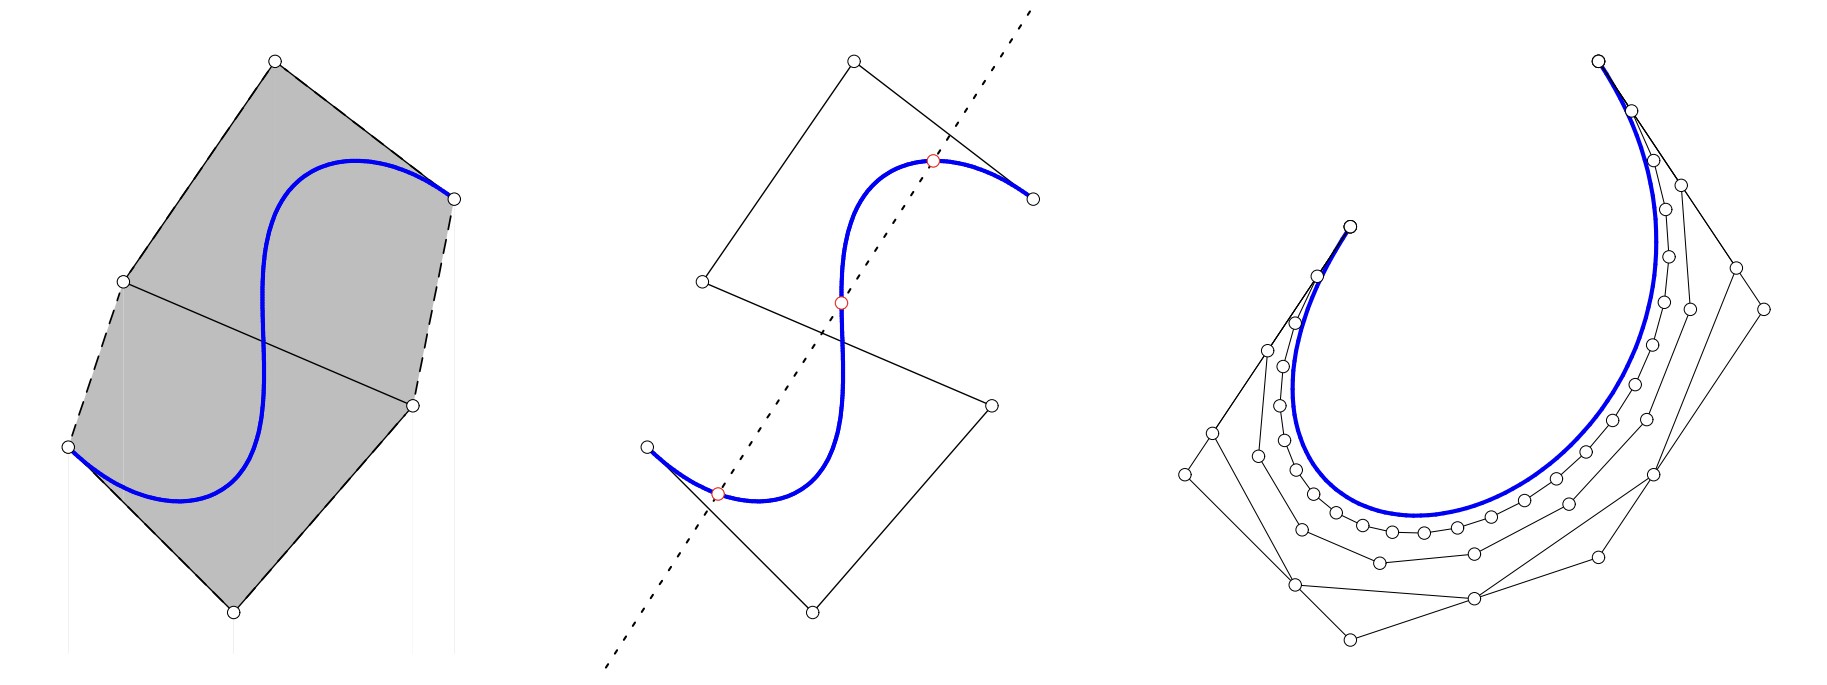
\includegraphics[width=\linewidth]{Slike/Bezier.png}
\end{subfigure}
\caption{Primer Bézierjeve krivulje in pripadajočega kontrolnega poligona. Na levi vidimo, da leži krivulja v svoji konveksni ogrinjači, na sredini je prikazana "Variation diminishing" lastnost, na desni pa je prikazano višanje reda krivulje.}
\label{fig:bezier}
\end{figure}
Pomemben primer so še racionalne Bézierjeve krivulje s pomočjo katerih lahko predstavimo še kompleksnejše objekte, npr. stožnice.
Definiramo jih z dodatnim seznamom uteži $W = (w_1, \dots , w_p)$.
Bazne funkcije racionalnih Bézierjevih krivulj definiramo kot:
\begin{equation}
r_k(t) = \frac{w_k b_k^p (t)}{\sum_{j=1}^p w_j b_j^p (t)},
\end{equation}
same krivulje pa potem spet dobimo kot linearno kombinacijo takih baznih funkcij, kjer koeficientom spet rečemo kontrolne točke. Navadne Bézierjeve krivulje lahko dobimo kot poseben primer, ko so vse uteži enake $1$. Geometrijsko lahko racionalno Bézierjevo krivuljo v $\mathbb{R}^d$ dobimo tako, da Bézierjevo krivuljo v $\mathbb{R}^{d+1}$ projeciramo na hiperravnino $x_{d+1}=1$.
\\
\\
Za konec omenimo še višje dimenzionalne objekte. Posplošitev na ploskve je enostavna - Bézierjovo ploskev dobimo s pomočjo tenzorskega produkta Bernsteinovih polinomov:
$S(u, v) = \sum_{i=1}^n \sum_{j=1}^m \textbf{B}_{i,j} b_i^p (u) b_j^q (v)$.
Pri tem se ohranijo omenjene lepe lastnosti Bézierovih krivulj, hkrati pa velja, da je rob take ploskve Bézierjeva krivulja. Analogno bi lahko definirali tudi racionalno Bézierovo ploskev.

\subsection{B Zlepki}
Do sedaj smo govorili o prostorih polinomov in vpeljali Bernsteinove polinome kot njihovo prikladno bazo. Z njihovo pomočjo smo tudi definirali Bézierjeve krivulje.
Veliko bolj bogati pa so prostori polinomskih zlepkov - ti vsebujejo funkcije izbranega reda gladkosti, ki so zožene na primerne intervale polinomi. Polinomi sami so seveda samo poseben primer polinomskih zlepkov.

B zlepki so baza tega prostora, ki ima lepe lastnosti, podobno kot so Bernsteinovi polinomi "lepa" baza za polinome.
V njihovi definicija igra pomembno vlogo seznam vozlov: $\Xi = ( \xi_1, \dots \xi_{n+p+1} )$, pri čemer se lahko kakšna vrednost vozla pojavi več kot enkrat (privzamimo še, da je seznam urejen nepadajoče). $p$ je red zlepka in $n$ izbrano število baznih funkcij za B-zlepke.

Zožen na interval med sosednjima, različnima vozloma je zlepek gladek (polinom $p$-te stopnje). Če vozel ni ponovljen, ima ob prehodu čezenj zlepek red gladkosti $C^{p-1}$. Splošneje, če je vozel ponovljen $m$ - krat, ima zlepek čezenj red gladkosti $C^{p-m}$. 
Ponavadi imamo opravka z odprtimi vozli - prvih in zadnjih $p+1$ vozlov ima isto vrednost. To povzroči, da so zlepki na robu interpolirajoči.

$k$-to bazno funkcijo stopnje $p$ označimo z $N_{k,p}(\xi)$. $N_{k,0}$ imajo enostavno obliko ($1$ na med sosednjima vozloma in $0$ sicer), višje stopnje pa dobimo rekurzivno s tako imenovano Cox-de Boor formulo.
Lastnosti $N_{k,p}(\xi)$ so sledeče:
\begin{itemize}
\item Particija enote $\sum_{k=1}^n N_{k,p}(\xi) = 1$.
\item nenegativnost $N_{k,p} \geq 0$.
\item Obstajajo eksplicitne formule za odvod/integral/višanje reda/dodajanje vozla.
\item Zlepek lahko numerično stabilno izračunamo z de Boor-ovim algoritmom.
\item Nosilec za bazno funkcijo B-zlepka reda $p$ je $p+1$ elementov: $\mathrm{supp} N_{k,p} \subset [\xi_k,\xi_{k+p+1}]$.
\item Ta baza je optimalna za primeren prostor zlepkov v podobnem smislu kot so Bernsteini optimalni za polinome.
\end{itemize}

\subsubsection{Krivulje iz B-Zlepkov}
Analogno z Bézierjovimi krivuljami lahko s pomočjo B-zlepkov tvorimo krivuljo $C(\xi)$. Koeficientom pred posameznimi baznimi B-zlepki spet rečemo kontrolne točke $\textbf{P}_k$.
\begin{equation}
 C(\xi) = \sum_{k=1}^n \textbf{P}_k N_{k,p}(\xi)
\end{equation}
Pridobljena krivulja interpolira le robne točke (pri odprtih vozlih), ter morebitne točke kjer je kratnost vozla enaka $p$. 
Lastnosti te krivulje so spet podobne kot pri Bézierovih krivuljah:
\begin{itemize}
\item Afine transformacije lahko namesto na krivulji uporabimo na kontrolnem poligonu.
\item Krivulja leži v konveksni ogrinjači kontrolnih točk.
\item Kot omenjeno krivulja interpolira na robu. Tangenta na vsakem robu je nosilka daljice, ki jo tvorita robni dve kontrolni točki.
\item Variation diminishing.
\item Zaradi lokalnega nosilca, sprememba kontrolne točke spremeni krivulje le v manjši okolici (za razliko od Bézierjevih krivulj).
\end{itemize}
Sedaj lahko definiramo trenutno enega najbolj razširjenih orodij v računalniški grafiki, sploh kar se inženirskih aplikacij tiče - NURBS (Non Uniform Rational B-Spline).
Podobno kot pri racionalnih Bézierjevih krivuljah, lahko definiramo bazne funkcije NURBSov kot:
\begin{equation}
R_{k,p} (\xi) = \frac{w_k N_{k,p} (\xi)}{\sum_{j=1}^n w_j N_{j,p}(\xi)}.
\end{equation}
V podrobne lastnosti NURBSov se na tej točki ne bomo spuščali in jih lahko bralec najde v npr. \cite{iso1}. Za nadaljno analizo bo zadostovala zgornja definicija. V praksi pogosto operiramo s še kompleksnejšimi objekti, ki jih pridobimo z leplenjem več NURBSov skupaj (tako imenovan multipatch NURBS), kjer na stičiščih zahtevamo, da velja določen pogoj gladkosti (zagotovo vsaj zveznost).

\section{Diskretizacija domene, katere rob je NURBS krivulja}

V nadaljevanju bomo privzeli, da imamo podano NURBS krivuljo:
\begin{equation}
C(\xi) = \sum_{k=1}^n \textbf{P}_k R_{k,p}(\xi),
\end{equation}
s čimer imamo v mislih, da imamo podan red krivulje $p$, kontrolne točke, uteži in vektor vozlov. Omejili se bomo na planarne krivulje, torej $\textbf{P}_k \in \mathbb{R}^2$.

Dodatno bomo zahtevali, da je krivulja zaprta ($C(b) = C(a)$, če je $C(\xi)$ definirana na $[a,b]$) ter enostavna ($\xi \to C(\xi)$ je injektivna).
Po Jordanovem izreku v tem primeru krivulja $C(\xi)$ loči prostor $\mathbb{R}^2$ na dva dela - notranjost $\Omega$ ter zunanjost $\bar{\Omega}^C$. Velja tudi, da je rob notranjosti slika krivulje $C(\xi)$, kar bomo označevali tudi z $\partial \Omega$.

Problem, ki ga želimo rešiti je naslednji - želimo diskretizirati množico $\Omega$.
Konkretno to pomeni, da hočemo algoritem, ki bo sprejel NURBS $C(\xi)$, ki opisuje $\partial \Omega$ in vrnil množico paroma različnih točk $X \subset \Omega$.
Od algoritma dodatno zahtevamo še, da ima eno izmed naslednjih možnosti:
\begin{itemize}
\item Algoritmu lahko podamo parameter $N$, ki določa število diskretizacijskih točk $N = |X|$.
\item Algoritmu lahko podamo parameter $h$, ki določa minimalno razdaljo med točkama iz $X$.
\end{itemize}
Parametra $N$ in $h$ nam določata finost naše diskretizacije.
\\
\\
Pridobljeno diskretizacijo lahko potem uporabimo za nadaljno numerično analizo na primer:
\begin{itemize}
\item Numerično reševanje parcialnih diferencialnih enačb na domeni $\Omega$ s pomočjo brezmrežnih metod.
\item Računanje integralov po domeni $\Omega$ s pomočjo metode (kvazi) Monte Carlo.
\end{itemize}
Pri obeh možnih aplikacijah je pomembno, da diskretizacijske točke $X$ enakomerno zapolnijo $\Omega$\footnote{Konkretneje, za reševanje PDE želimo, da so točke kvazienakomerno porazdeljene, za Monte Carlo pa da so kvazinaključne. Ti lastnosti nista čisto enaki, vendar se v podrobnosti ne bomo spravljali.}. Želimo, da naša diskretizacija $X$ ne pušča preveč lukenj - da radij največje krogle v $\Omega$, ki ne vsebuje točk iz $X$ z večanjem $N$ (ali manjšanjem $h$) relativno hitro pada.
\\
\\
V kontekstu bremrežnega reševanja parcialnih diferencialnih enačb pogosto dodatno zahtevamo še tri pogoje:
\begin{itemize}
\item Razdalja med poljubnima različnima točkama iz $X$, naj bo večja od neke predpisane minimalne razdalje.
\item Preko celotne domene $\Omega$, naj razdalja med najbližjima sosedoma (iz $X$) ne varira preveč.
\item Diskretizacija $X$ mora vsebovati tudi robne točke na $\partial \Omega$, oziorma mora biti kompatibilna z obstoječo diskretizacijo roba.
\end{itemize}
Prva pogoja pripomoreta k stabilnosti brezmrežnih metod, tretji pa je potreben, če želimo natančno upoštevati robne pogoje danih problemov.
\\
\\
V nadaljevanju bomo predstavili dva možna pristopa za diskretizacijo $\Omega$.
\subsection{inRS - algoritem za določanje notranjosti domene, omejene z NURBS}
Prvi način bo slonel na algoritmu inRS, ki sta ga predstavila Sommarive in Vianello \cite{inrs}.
inRS je algoritem, s katerim lahko za dano $\Omega$ izračunamo indikatorsko funkcijo $1_\Omega(\textbf{x})$, ki je enaka $1$, če $\textbf{x} \in \Omega$ in $0$ sicer.
\\
\\
Ideja algoritma je sledeča znano dejstvo - Če iz točke $\textbf{x}$ potegnemo poltrak in preštejemo presečišča z $\partial \Omega$ in jih je liho število je $\textbf{x}$ v domeni, sicer pa ne.

Poseben primer, kjer to zelo dobro deluje je, če je rob $\partial \Omega$ poligon (tudi nekonveksen). To je pravzaprav poseben primer, ko imamo opravka s krivljo B-zlepkov stopnje $1$. Zaradi enostavne oblike $\partial \Omega$ lahko v tem primeru presečišča enostavno izračunamo, treba je le paziti na posebne primere, ko npr. poltrak sovpada s katero od stranic poligona ali se dotakne enega izmed vogalov. Takšnih primerov se lahko vedno ognemo, saj se pojavijo le pri končnem številu poltrakov.
\\
\\
V našem primeru je $\partial \Omega$ slika NURBSa:
\begin{equation}
C(\xi) = \frac{\sum_{k=1}^n \textbf{P}_k w_k N_{k,p}(\xi)}{\sum_{k=1}^n w_k N_{k,p}(\xi}.
\end{equation}

Definicijsko območje NURBSa je dano - interval $I$. Vemo, da ta interval razpade na podintervale $\{I_k \}_k$, tako, da za vsak $k$ velja $C(\xi)|_{I_k} = (\alpha_k(\xi), \beta_k(\xi))$, kjer sta $\alpha_k$ in $\beta_k$ racionalni funkciji. Ti intervali so oblike $[\xi_i,\xi_{i+1}]$, kjer sta $\xi_i$ in $\xi_{i+1}$ paroma različna vozla. Ker vemo, da so B-zlepki na takem intervalu kar polinomi, je NURBS zoožen na interval kar par (ker so kontrolne točke v $\mathbb{R}^2$) racionalnih funkcij.


Sedaj bomo vsakega izmed $I_k$ še nadaljno razbili na podintervale $I_{k,j}$. V ta namen (razlog bo postal jasen v kratkem) moramo izračunati ničle $\alpha_k'(\xi), \beta_k'(\xi)$. Če pišemo $\alpha_k(\xi) = u_k(\xi)/v_k(\xi)$ in $\beta_k(\xi) = w_k(\xi)/z_k(\xi)$ to pomeni, da moramo za vsak $k$ rešiti polinomski enačbi:
\begin{align}
&u_k'(\xi) v_k(\xi) - u_k(\xi) v_k'(\xi) = 0. \\
&w_k'(\xi) z_k(\xi) - w_k(\xi) z_k'(\xi),
\end{align}
kar je dobro znan problem za katerega obstajajo učinkoviti numerični postopki. Avtorji članka so na primer, uporabili kar MATLAB roots funkcijo, ki izračuna ničle polinoma s pomočjo računanja lastnih vrednosti pridružene matrike. Vse izračunane ničle postanejo krajišča novih intervalov $I_{k,j}$. 

Za fiksen $k$ so $\alpha_k(\xi), \beta_k(\xi)$ zoožene na $I_{k,j}$ konstante ali monotone funkcije, slika NURBSa, zoženega na ta interval pa je vsebovana v pravokotniku:
\begin{align}
&B_{k,j} = [a_{k,j}, b_{k,j}] \times [c_{k,j}, d_{k,j}], \\
& a_{k,j} = \mathrm{min}_{\xi \in I_{k,j}} \alpha_k(\xi), \\
& b_{k,j} = \mathrm{max}_{\xi \in I_{k,j}} \alpha_k(\xi), \\
& c_{k,j} = \mathrm{min}_{\xi \in I_{k,j}} \beta_k(\xi), \\
& d_{k,j} = \mathrm{max}_{\xi \in I_{k,j}} \beta_k(\xi), 
\end{align}
ki ga bomo imenovali "monotoni pravokotnik".
Unija le-teh po vseh $k,j$ pokrije $\partial \Omega$, znotraj vsakega pa je NURBS monotona funkcija.
Primer, ko je NURBS ne le monotona, ampak konstantna funkcija ustreza pravokotniku z "ničelno širino" in ga obravnavamo posebej.
Primer pokritij $\partial \Omega$ z monotonimi pravokotniki je prikazan na Sliki \ref{fig:pokritje}.
\begin{figure}[H]
\centering
\begin{subfigure}{.8\textwidth}
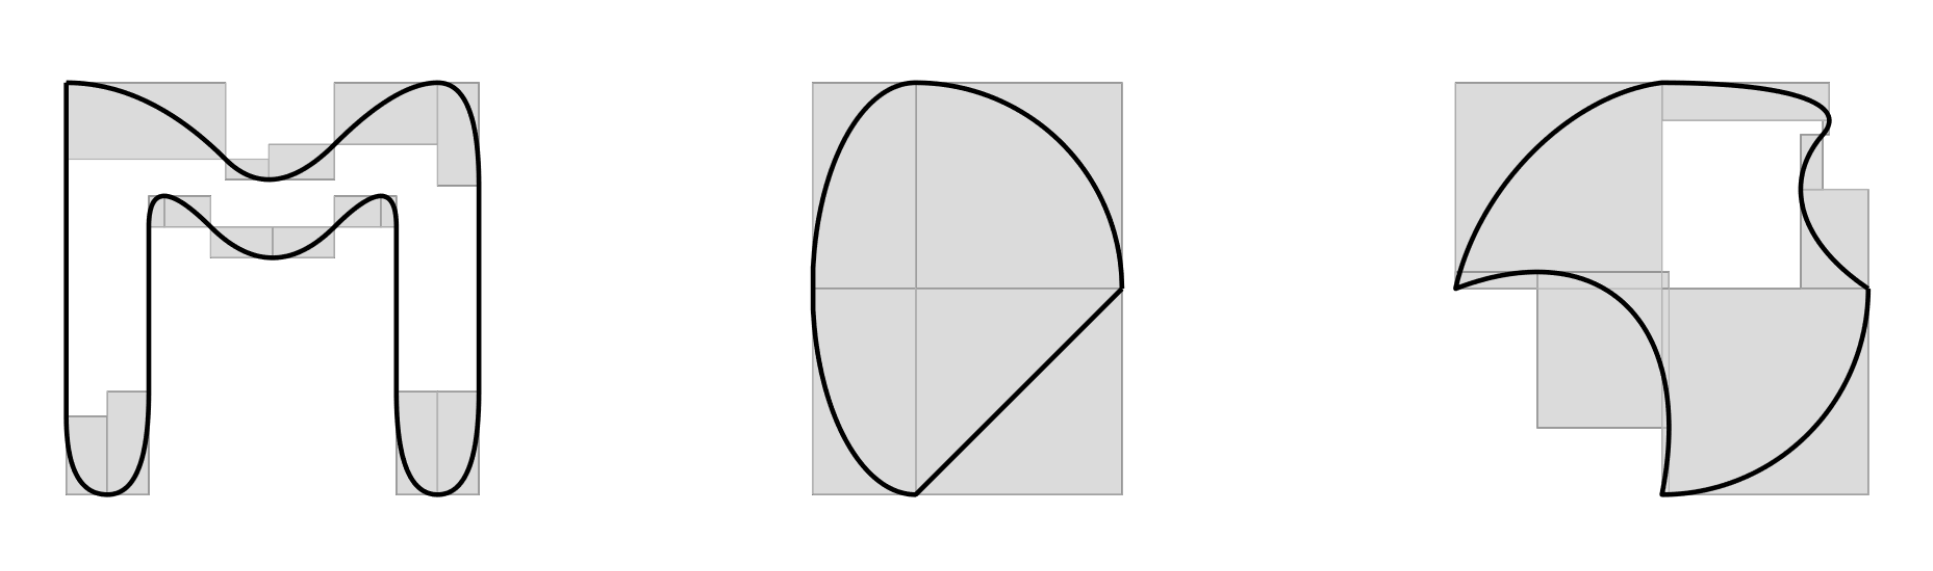
\includegraphics[width=\linewidth]{Slike/inRS_pokritje.png}
\end{subfigure}
\caption{Primeri treh planarnih NURBS krivulj in pripadajočih monotonih pravokotnikov. Na levi sliki imamo vzdolž vertikalnih "stranic" pravokotnike širine nič.}
\label{fig:pokritje}
\end{figure}
Definirajmo še globalni mejni pravokotnik, v katerem leži celotna $\partial \Omega$. To je enostavno, saj bodo vogali globalnega pravokotnika sovpadali z vogalom enega izmed monotonih.
\\
\\
Iskanje monotonih pravokotnikov je bil preprocessing korak algoritma inRS. Sedaj lahko za dano točko povemo, ali je znotraj $\Omega$.
Recimo, da opazujemo točko $(x_0,y_0)$. Če leži zunaj globalnega mejnega pravokotnika je očitno $(x_0,y_0) \notin \Omega$.
V kolikor je znotraj globalnega mejnega pravokotnika, bomo uporabili podobno idejo kot v primeru poligonov.
Oglejmo si poltrak $\{(x_0,y) , y \leq y_0\}$. Tak poltrak bo sekal monotone pravokotnike $B_{k,j}$ za katere velja 
\begin{equation}
a_{k,j} \leq x_0 \leq b_{k,j} , y_0 \geq c_{k,j}.
\end{equation}
V kolikor za nek $k,j$ velja tudi $y_0 > d_{k,j}$, lahko število presečišč povečamo za ena, saj ima poltrak zagotovo eno presečišče s krivuljo v monotonem pravoktoniku $B_{k,j}$.
V nasprotnem primeru, če za $k,j$ velja $y_0 \leq d_{k,j}$, lahko obstoj presečišča preverimo spet z rešitvijo polinomske enačbe:
\begin{equation}
u_k (\xi) - x_0 v_k (\xi) = 0,
\end{equation}
kar nam da rešitev $\xi_0$. Preveriti moramo še, da zanjo velja $\beta_{k}(\xi_0) \leq y_0$. 
Če je število vseh presečišč liho je potem $(\bar{x},\bar{y})$ znotraj $\partial \Omega$, sicer pa ne.

Paziti moramo še na morebitne posebne primere. V kolikor se zgodi, da ta poltrak sovpada z robom enega izmed monotonih pravokotnikov, postopek ponovimo z horizontalnim poltrakom. V redkem primeru, ko se težava ponovi, lahko notranjost za problematično točko določimo tudi preko ovojnega števila:
\begin{equation}
\nu((x_0,y_0) = \frac{1}{\mathrm{length}(I)} \sum_k \int_{I_k} \frac{\beta_k'(\xi) (\alpha_k(\xi) - x_0)-\alpha_k'(\xi) (\beta_k(\xi)-y_0)}{(\alpha_k(\xi)-x_0)^2 + (\beta_k(\xi)-y_0)^2} \textup{d}\xi,
\end{equation}
kjer vse integrale izračunamo numerično s pomočjo npr. kvadraturne formule. Pri tem dovolimo napako do $0.5$, saj vemo, da mora bit rezultat celo število. Točka je potem v notranjosti $\Omega$, če in samo če je ovojno število liho.
\\
\\
Algoritem lahko potencialno pospešimo, če intervale $I_{k,j}$ še nadaljno razdelimo. S tem pravotkoniki postajajo manjši in že sami po sebi bolje opisujejo krivuljo. Ker so manjši, za več točk velja, da ne bodo vsebovane v nobenem izmed njih in bo torej algoritem hitrejši (za manj točk bo treba reševat polinomsko enačbo). Primer nadaljne subdivizije pravokotnikov je prikazan na Sliki \ref{fig:pokritjeFino}.
\begin{figure}[H]
\centering
\begin{subfigure}{.8\textwidth}
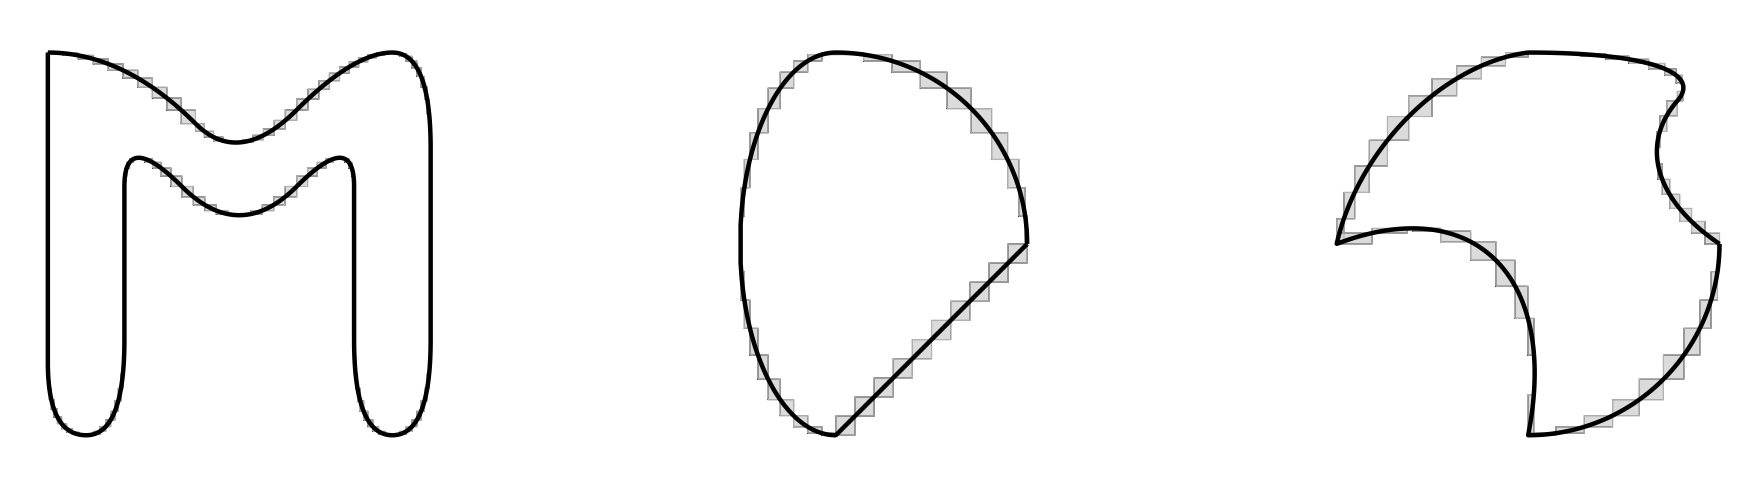
\includegraphics[width=\linewidth]{Slike/inRS_pokritje_fino.png}
\end{subfigure}
\caption{Prejšnje tri NURBS krivulje, tokrat s finejšim pokritem s pravokotniki.}
\label{fig:pokritjeFino}
\end{figure}
Ko imamo indikatorsko funkcijo $1_\Omega$, lahko diskretizacijo domene $\Omega$ enostavno dobimo s pomočjo vzorčenja z zavračanjem.
Kvazienakomerna zaporedja, ki diskretizirajo kvadrat, so namreč dobro znana, npr. pari Haltonovih zaporedij.
Za naš kvadrat vzamemo kar globalen mejen pravokotnik (po potrebi skaliran do kvadrata) in zanj poženemo enega izmed generatorjev kvazienakomernih zaporedij. Z algoritmom inRS preverimo, ali je trenutni kandidat res v notranjosti $\Omega$. Če je, ga dodamo naši diskretizaciji $X$, sicer pa ga zavržemo. Postopek ponavljamo, dokler ne dobimo v $X$ želenega števila točk. Primer je na sliki \ref{fig:inRSrezultat}.
\begin{figure}[H]
\centering
\begin{subfigure}{.8\textwidth}
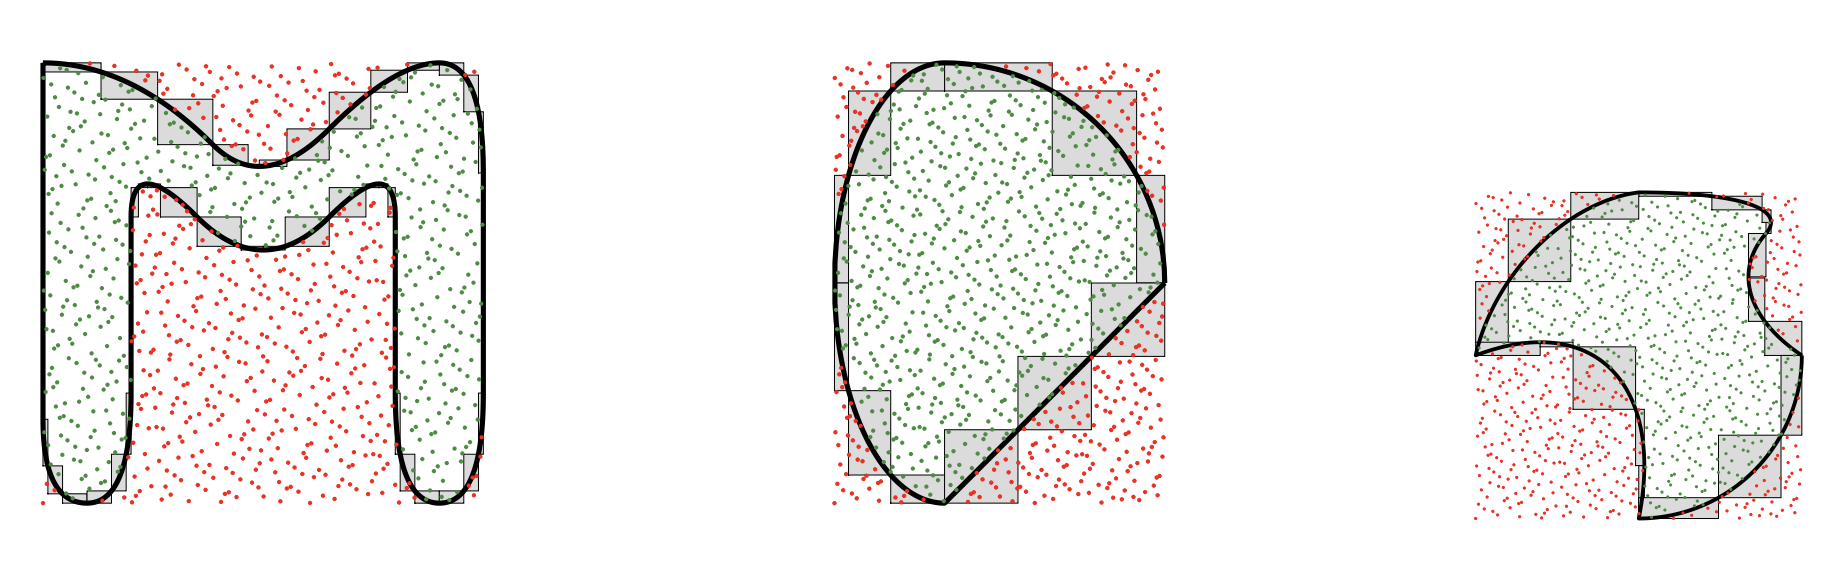
\includegraphics[width=\linewidth]{Slike/inRS_rezultat.png}
\end{subfigure}
\caption{Diskretizacija notranjosti prejšnjih treh krivulj s pomočjo Haltonovih kvazienakomernih zaporedij in vzorčenja z zavračanjem. Zelene točke predstavljajo diskretizacijo, rdeče pa zavržene kandidate.}
\label{fig:inRSrezultat}
\end{figure}
Za konec omenimo, da lahko algoritem uporabimo tudi za primer, ko je $\partial \Omega$ multipatch NURBS. V tem primeru si lahko predstavljamo, da imamo še en nivo razbitja intervala $I_{n,k,j}$, kjer se zdaj prvi indeks nanaša na indeks posamezne NURBS krivulje. Preostanek algoritma poteka analogno.
\subsection{NURBS-DIVG algoritem za diskretizacijo}
Poglejmo še en način diskretizacije objektov $\Omega$, katerih rob lahko opišemo z NURBS. Algoritem, ki ga bomo tu opisali je precej drugačen od prejšnjega v smislu, da poglavitni del ne bo algoritem za izračun indikatorske funkcije $1_\Omega$, ampak je algoritem tipa "advancing front", kjer se diskretizacija sekvenčno širi od podanih začetnih točk.

Ta algoritem so zasnovali sodelavci na odseku E6 na IJS in je v člankih formuliran v poljubno dimenzijah, zato bomo to formulacijo uporabljali tudi tukaj. Seveda se lahko vedno omejimo na omenjen primer, ko je $\partial \Omega$ krivulja.

Algoritem bomo predstavili v več korakih. Najprej osnovno verzijo algoritma DIVG, ki diskretizira $\Omega$, v primeru, ko je $\partial \Omega$ že diskretizrian, potem algoritem sDIVG, ki je posplošitev na diskretizacijo parametrično podanih objektov in končno algoritem NURBS-DIVG, ki bo ustrezal naši želeni diskretizaciji.
\subsubsection{DIVG}
Za začetek se omejimo na poenostavljen primer, ko imamo že na voljo funkcijo, ki nam za dano točko pove, ali je v domeni $\Omega$ ali ne. Poleg tega pa imamo podanih nekaj začetnih (seed) točk diskretizacije $X$. Te so ponavadi diskretizacija roba $\partial \Omega$, vendar jih imamo lahko tudi v domeni. Algoritem DIVG začetne točke skupaj z želeno diskretizacijsko dolžino $h$ "zapolni" do diskretizacije celotne $\Omega$ \cite{divg}.
\\
\\
Začnemo tako, da vse začetne točke zložimo v vrsto (podatkovno strukturo - queue). To je vrsta trenutno aktivnih točk s pomočjo katerih bomo generirali nove. Algoritem se izvaja dokler bo ta vrsta neprazna.

Na vsakem koraku algoritma vzamemo element iz vrste trenutno aktivnih točk, recimo mu $\textbf{x}$. Na krožnici (oziroma v višjih dimenzijah, sferi) s centrom $\textbf{x}$ in radijem $h$ nato generiramo kandidate za dopolnitev diskretizacije\footnote{Diskretizacija sfere ni komplicirana. Za krožnico lahko, na primer damo prvo točko k $\varphi = 0$ in jih potem sekvenčno dodajamo za $h$ narazen po krožnici, dokler še lahko.}. V kontekstu brezmrežnih metod se izkaže, da prevelika regularnost diskretizacije slabo vpliva na stabilnost, zato kandidate na sferi še zarotiramo za naključen kot. Vsakega izmed novih kandidatov dodamo v diskretizacijsko množico $X$ (in v vrsto trenutno aktivnih točk), če velja, da je znotraj domene $\Omega$ in je hkrati od vseh ostalih točk v $X$ oddaljen za najmanj $h$. Potek algoritma je viden na Sliki \ref{fig:divg}.

\begin{figure}[H]
\centering
\begin{subfigure}{.8\textwidth}
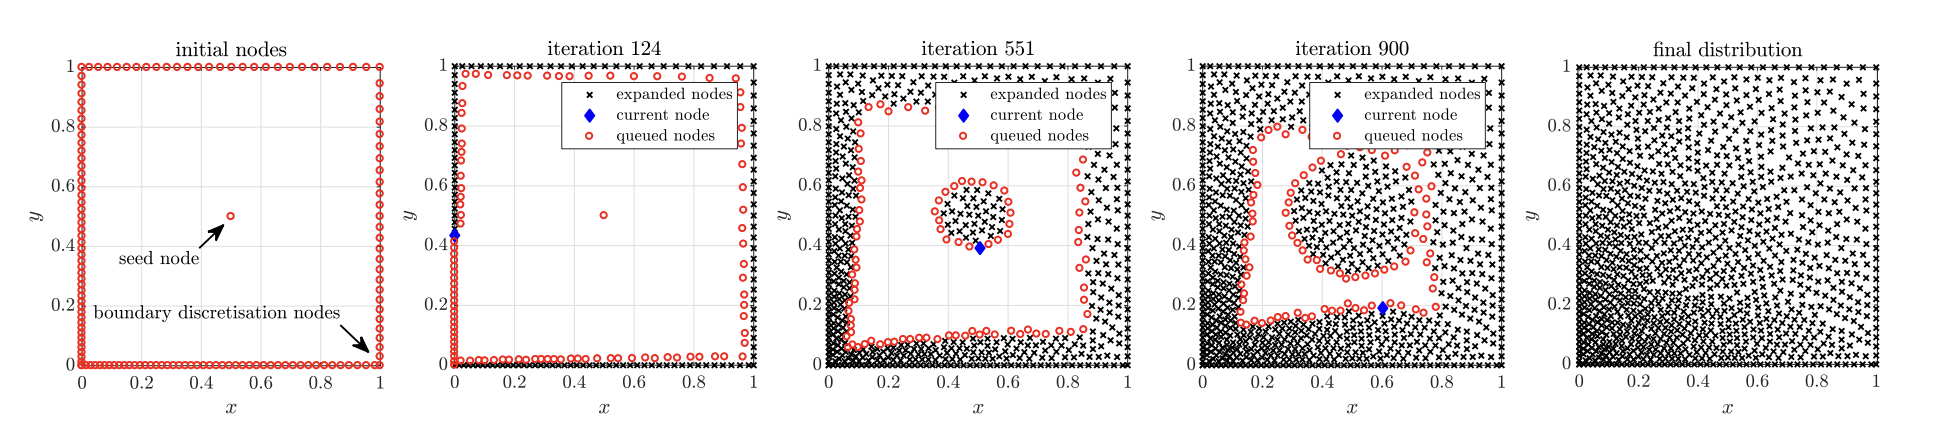
\includegraphics[width=\linewidth]{Slike/divg.png}
\end{subfigure}
\caption{Diskretizacija kvadrata z DIVG algoritmom. Začetne točke so na robu ter ena v sredini domene, nakar jih algoritem postopoma dodaja. Na sliki je sicer prikazan poseben primer, ko je $h$ krajevno odvisen.}
\label{fig:divg}
\end{figure}
Učinkovitost predstavljenega algoritma lahko izboljšamo s pomočjo podatkovne strukture kd-drevesa, katere namen je učinkovito iskanje najbližjih sosedov iz dane možice točk. S tem precej pospešimo preverjanje, ali je trenutni kandidat dovolj oddaljen od obstoječih točk.
\\
\\
Algoritem DIVG, kot je tukaj predstavljen verjetno ne deluje kot nič posebnega, saj smo privzeli, da imamo dano funkcijo, ki nam pove ali smo v notranjosti domeni, hkrati pa imamo danih že nekaj začetnih točk. V nadaljevanju se bomo teh problemov znebili, vendar vseeno omenimo, zakaj je algoritem DIVG kljub temu uporaben. Primeren je za diskretizacija enostavnejših objektov, kjer pa je lahko diskretizacijska razdalja $h$ krajevno odvisno (pri vsakem koraku algoritma moramo pač namesto konstantega $h$, vzeti $h$, ki pripada dani točki). Krajevno odvisne diskretizacijske razdalje sicer niso predmet naše obravnave, zato se vanje ne bomo poglabljali.

\subsubsection{sDIVG}
Algoritem sDIVG \cite{sdivg} je posplošitev algoritma DIVG na parametrično podane domene. Z njegovo pomočjo bomo diskretizirali rob $\partial \Omega$, nakar bomo to diskretizacijo uporabili za diskretizacijo $\Omega$ po navadnem algoritmu DIVG. Parametrično ploskev (oz. krivuljo) imamo podano kot funkcijo $\textbf{r}: \Xi \to \partial \Omega$. Za algoritem sDIVG bomo potrebovali tudi Jacobian $\nabla \textbf{r}$.
\\
\\
Kot prej bomo potrebovali neko množico začetnih točk, vendar bodo ti živeli v prostoru $\Xi$. V kolikor jih ni, se začetne točke vzame naključno. Ker tokrat populiramo sam rob, ni nobene potrebe, da bi začetne točke bile na robu $\Xi$. Začetne točke lahko enostavno generiramo, ker je v praksi prostor $\Xi$ enostaven, na primer interval ali pravokotnik. 

Glavna ideja algoritma sDIVG je uporaba algoritma DIVG v prostoru $\Xi$. Kot prej bomo trenutno aktivne točke iz prostora $\Xi$ imeli v vrstni podatkovni strukturi. Recimo, da trenutmo generiramo nove kandidate s pomočjo $\boldsymbol{\xi} \in \Xi$. Ti bodo spet iz sfere, centrirani na $\boldsymbol{\xi}$.  V primeru DIVG je ta sfera imela predpisan radij $h$. Pri parametričnih domenah to ni več primerna izbira, saj točke na razdalji $h$ v prostoru $\Xi$ niso nujno na razdalji $h$ zatem, ko jih preslikamo v prostor $\partial \Omega$.
Zapišimo tipičnega kandidata kot $\boldsymbol{\xi} + \alpha \textbf{s}$, kjer je $\textbf{s}$ enotski vektor. Želimo:
\begin{equation}
||\textbf{r}(\boldsymbol{\xi}) - \textbf{r}(\boldsymbol{\xi} + \alpha \textbf{s})|| = h
\end{equation}
Oceno za parameter $\alpha$ dobimo z linearnim približkom: $\textbf{r}(\boldsymbol{\xi}+\alpha \textbf{s}) \approx \textbf{r}(\boldsymbol{\xi}) + \alpha \nabla \textbf{r}(\boldsymbol{\xi}) \textbf{s}$.
Pri generaciji kandidatov okoli $\boldsymbol{\xi}$ bomo torej za dano smer $\textbf{s}$ izbrali kandidata $\boldsymbol{\xi} + \alpha \textbf{s}$, kjer je $\alpha = h/||\nabla \textbf{r}(\boldsymbol{\xi}) \textbf{s}||$. Pogosto privzamemo, da je parametrizacija $\textbf{r}(\boldsymbol{\xi})$ regularna in se tako znebimo primerov, kjer bi bila takšna izbira $\textbf{s}, \alpha$ nemogoča.
Podobno kot pri DIVG nove kandidate $\boldsymbol{\xi}^\prime$ sprejmemo le, če je $\textbf{r}(\boldsymbol{\xi}^\prime)$ dovolj daleč od ostalih točk in, če $\textbf{r}(\boldsymbol{\xi}^\prime) \in \partial \Omega$. Slednje je enostavno preverljivo, saj zadošča preveriti, ali $\boldsymbol{\xi}^\prime \in \Xi$. Za preverjanje razdalje do ostalih točk spet uporabimo kd-drevo, ki ga tokrat gradimo na točkah iz $\partial \Omega$.
Primer delovanja algoritma je prikazan na Sliki \ref{fig:sdivg}.
\begin{figure}[H]
\centering
\begin{subfigure}{.8\textwidth}
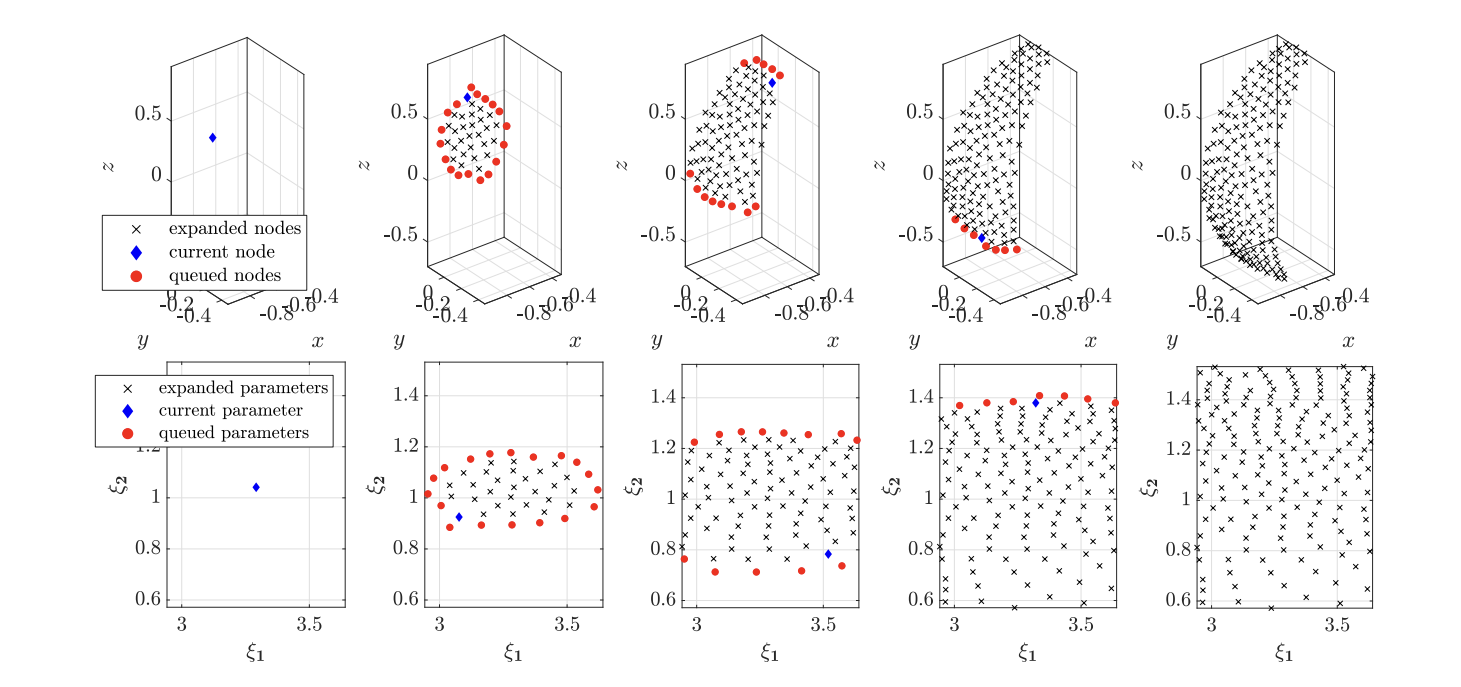
\includegraphics[width=\linewidth]{Slike/sdivg.png}
\end{subfigure}
\caption{Potek algoritma sDIVG v prostoru $\partial \Omega$ (zgoraj) in prostoru $\Xi$ (spodaj).}
\label{fig:sdivg}
\end{figure}
Kot zanimivost povejmo še, da algoritem deluje tudi, če je $\partial \Omega$ sebe sekajoča. Primer tega je viden na Sliki \ref{fig:sdivgRoman}.
\begin{figure}[H]
\centering
\begin{subfigure}{.8\textwidth}
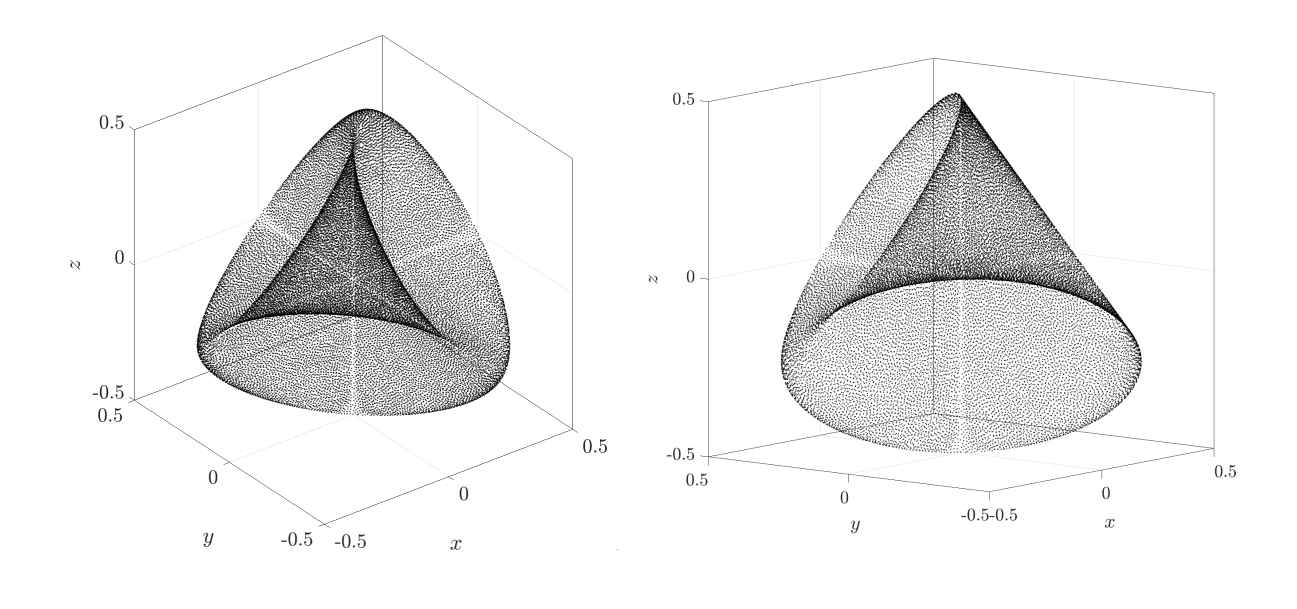
\includegraphics[width=\linewidth]{Slike/sdivgRoman.png}
\end{subfigure}
\caption{Rimska ploskev, diskretizirana s sDIVG.}
\label{fig:sdivgRoman}
\end{figure}
\subsubsection{NURBS-DIVG}
sDIVG, predstavljen v prejšnjem poglavju deluje za poljubne parametrične krivulje $\partial \Omega$, torej tudi za NURBS.
V tem razdelku bomo še dokončno povedali kako diskretiziramo še notranjost $\Omega$. To bo algoritem NURBS-DIVG \cite{nurbsdivg}.

Najprej povejmo, kako postopamo, če imamo multipatch NURBS-ov. Torej, če je $\partial \Omega$ unija več $\partial \Omega_i$. Avtorji algoritma so se odločili za naslednji postopek: Najprej diskretiziramo preseke NURBS patchev. Če imamo opravka s krivuljo so to zgolj točke, ki jih enostavno dodamo v diskretizacijo, v primeru NURBS ploskev pa so preseki NURBS krivulje, za katere uporabimo sDIVG algoritem. Zatem diskretiziramo še vsakega $\partial \Omega_i$ posebej, spet z sDIVG algoritmom, kjer za začetne točke vzamemo točke iz diskretiziranih presekov. To je prikazano na Sliki \ref{fig:nurbsmultipatch}.
\begin{figure}[H]
\centering
\begin{subfigure}{.8\textwidth}
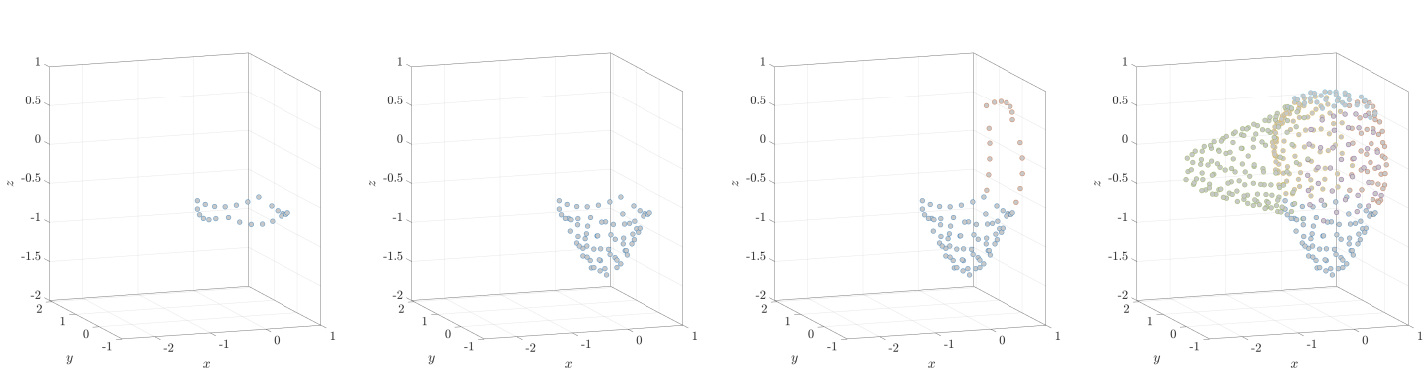
\includegraphics[width=\linewidth]{Slike/nurbsmultipatch.png}
\end{subfigure}
\caption{Diskretizaciji deformirane sfere, sestavljene iz petih NURBSev. Najprej diskretiziramo NURBS krivuljo na preseku dveh NURBS ploskev potem pa se posamezne ploskve.}
\label{fig:nurbsmultipatch}
\end{figure}
Naslednje vprašanje je, kako diskretiziramo še notranjost domene $\Omega$. Ker smo rob že diskretizirali, bi v ta namen radi uporabili navaden DIVG algoritem, kjer diskretiziran rob vzamemo za začetne točke. Vendar pa potrebujemo še indikatorsko funkcijo za $\Omega$.
\\
\\
Tudi aproksimacijo indikatorske funkcije bomo dobili s pomočjo diskretiziranega roba. Ker imamo poleg parametrizacije na voljo tudi Jacobian, lahko za vsako točko na robu izračunamo tudi normalo. Recimo, da nas zanima ali je točka $\textbf{x}$ v domeni $\Omega$. Prvi korak je poiskati tisto točko $\textbf{p} \in \partial \Omega$, ki je najbližje $\textbf{x}$. Označimo z $\textbf{n}$ navzven orientirano normalo v točki $\textbf{p}$. Hiter geometrijski premislek pove, da je $\textbf{x}$ znotraj domene, če velja:
\begin{equation}
\textbf{n} \cdot (\textbf{x} - \textbf{p}) < 0.
\end{equation}
V praksi je težko poiskati najbližjo točko na $\partial \Omega$, zato bomo za $\textbf{p}$ vzeli, točki iz diskretizacije roba $\partial \Omega$, ki je najbližja točki $\textbf{x}$. To lahko učinkovito najdemo s pomočjo kd drevesa. Seveda pa je to zgolj aproksimacija za indikatorsko funkcijo in je lahko nenatančna, če je rob preslabo diskretiziran. V ta namen pogosto "supervzorčimo" - rob diskretiziramo za nek faktor ($2-5$) gosteje kot je potrebno, izključno za namene boljše aproksimacije indikatorske funkcije. Primer tega je na Sliki \ref{fig:supersampling}.
\begin{figure}[H]
\centering
\begin{subfigure}{.48\textwidth}
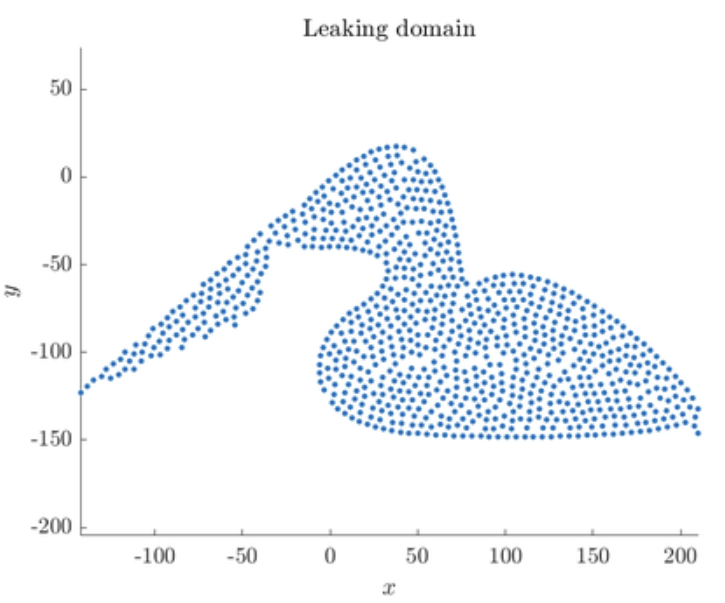
\includegraphics[width=\linewidth]{Slike/supersampling1.png}
\end{subfigure}
\begin{subfigure}{.48\textwidth}
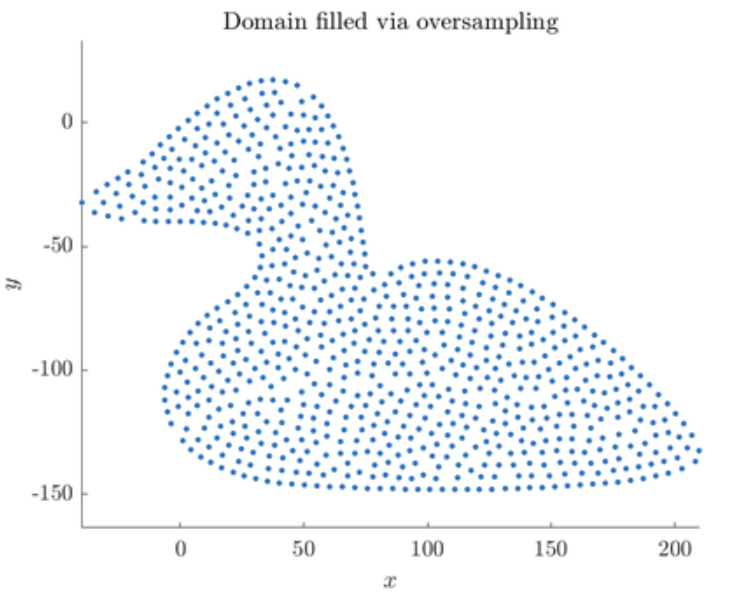
\includegraphics[width=\linewidth]{Slike/supersampling2.png}
\end{subfigure}
\caption{Na levi je primer diskretizacije $\Omega$ v obliki račke, kjer točke zunaj "kljuna" napačno identificiramo kot notranje. Na desni smo problem rešli s pomočjo supervzorčenja roba.}
\label{fig:supersampling}
\end{figure}
Sedaj imamo vse komponente, ki jih potrebujemo za DIVG algoritem in s tem diskretizacijo domene $\Omega$. 
Končajmo to sekcijo z nekaj dodatnimi primeri algoritma NURBS-DIVG. Ti so na Slikah \ref{fig:primeri} \ref{fig:cog} \ref{fig:geko}.
\begin{figure}[H]
\centering
\begin{subfigure}{.8\textwidth}
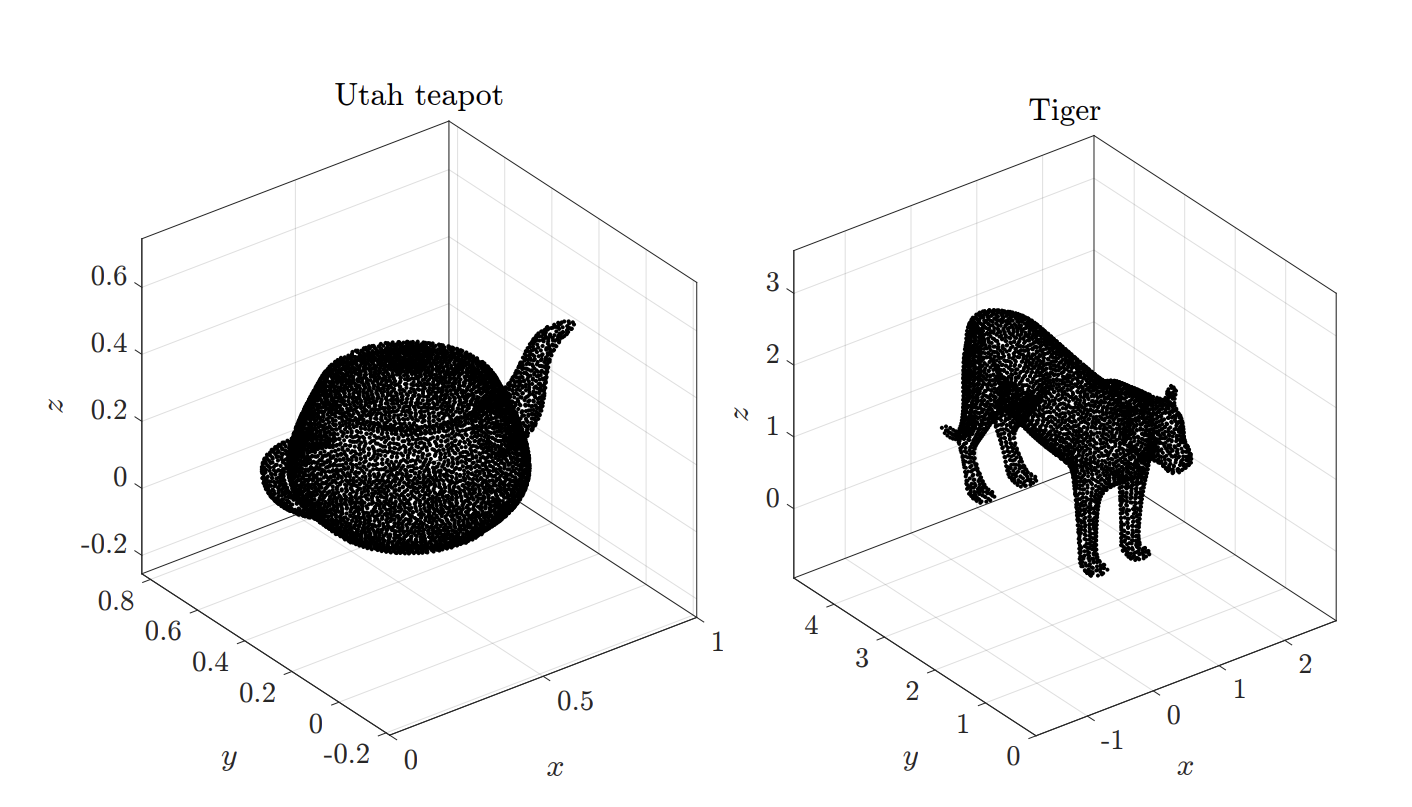
\includegraphics[width=\linewidth]{Slike/primeri.png}
\end{subfigure}
\caption{Diskretizacija Utah čajnika (32 patchev, 7031 točk) in tigra (124 patchev, 4753 točk) s NURBS-DIVG.}
\label{fig:primeri}
\end{figure}

\begin{figure}[H]
\centering
\begin{subfigure}{.6\textwidth}
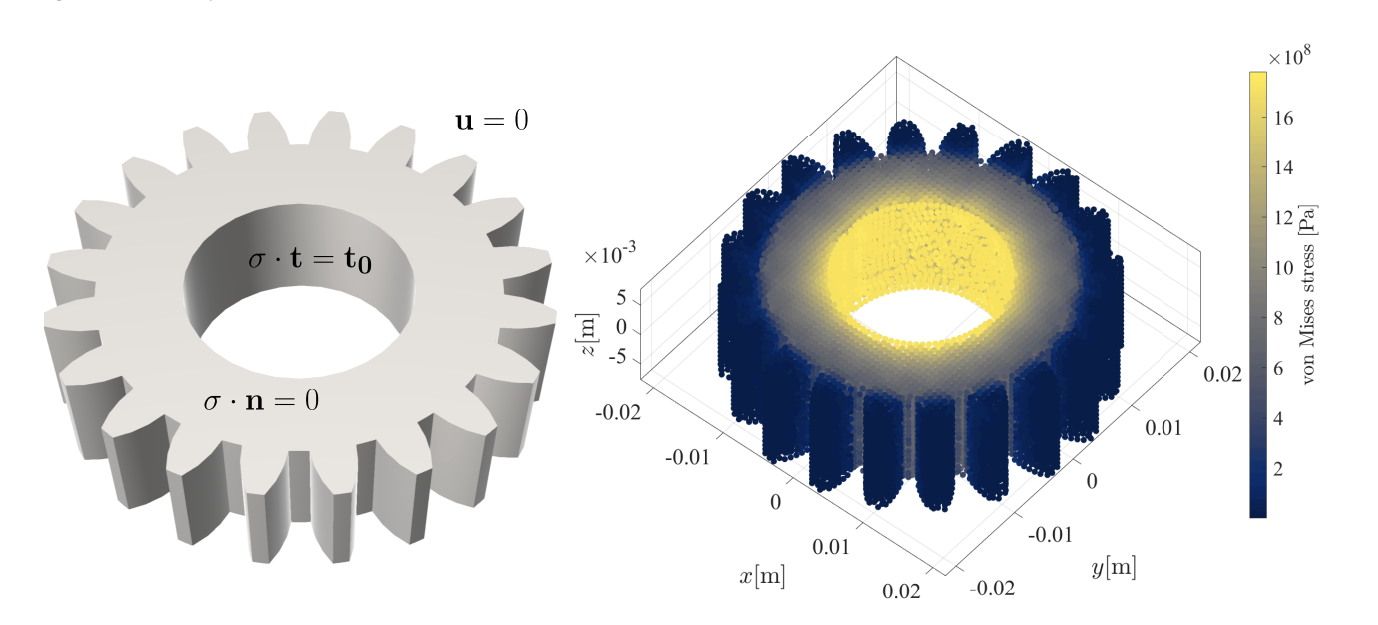
\includegraphics[width=\linewidth]{Slike/cog.png}
\end{subfigure}
\caption{Diskretizacija zobnika ter brezmrežna rešitev enačb linearne elastičnosti v njem.}
\label{fig:cog}
\end{figure}

\begin{figure}[H]
\centering
\begin{subfigure}{.5\textwidth}
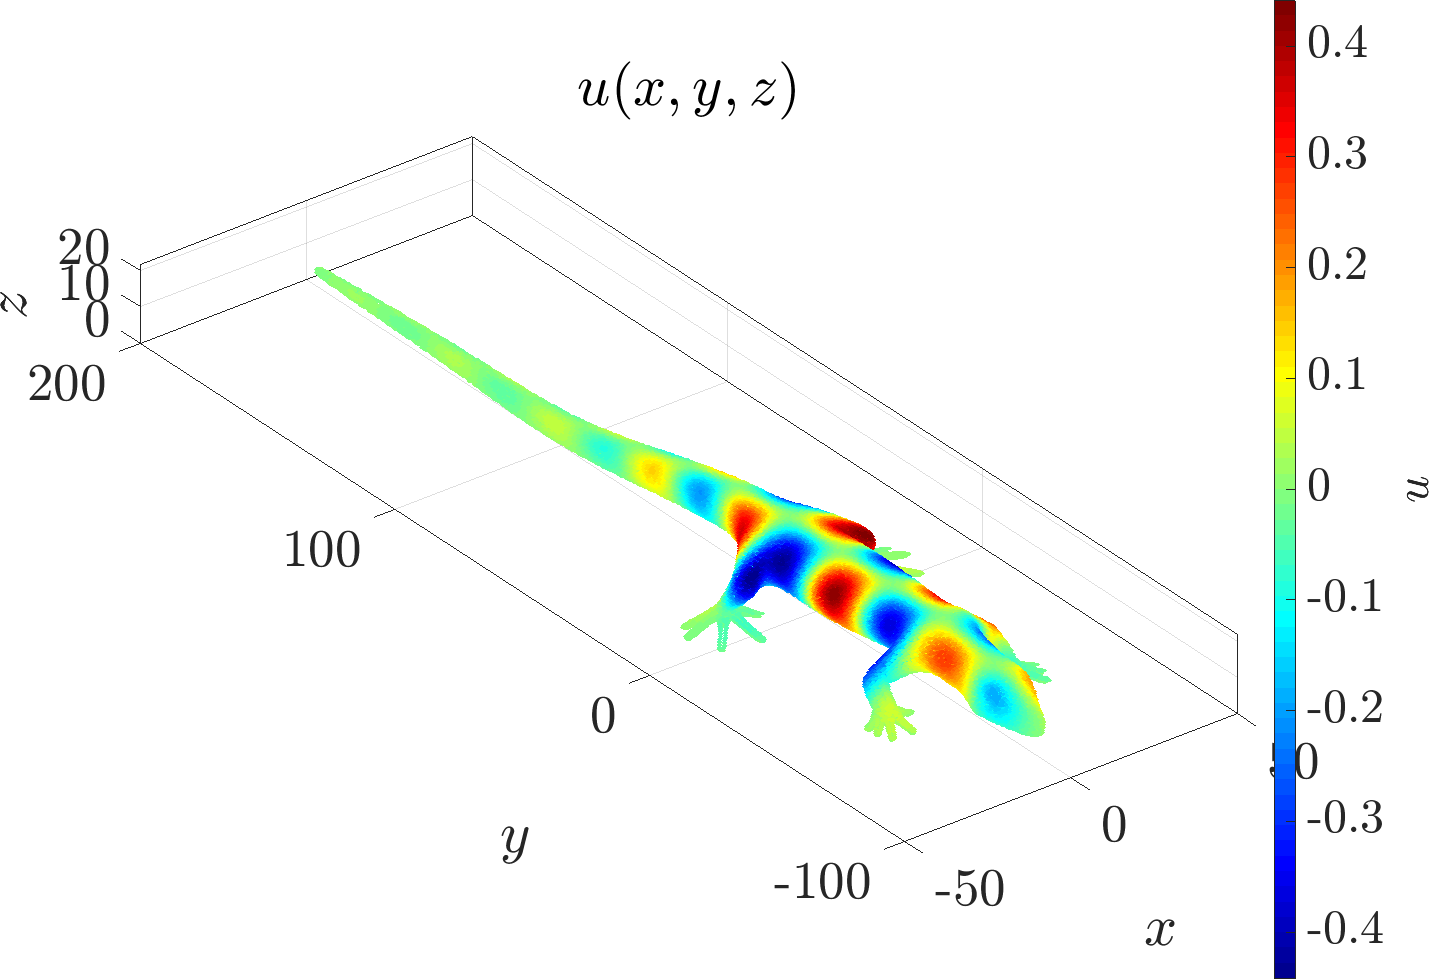
\includegraphics[width=\linewidth]{Slike/geko.png}
\end{subfigure}
\caption{Diskretizacija kuščarja (128 patchev) ter rešitev Poissonove enačbe v njem.}
\label{fig:geko}
\end{figure}
\subsection{Primerjava}
Opisali smo dva pristopa za diskretizacijo domen, katerega rob so (patchi) NURBS krivulj.
Za konec povzamimo glavne razlike med njima:
\begin{itemize}
\item inRS deluje samo v 2D, medtem ko se NURBS-DIVG enostavno posploši na višje dimenzije.
\item inRS operira samo s številom točk $N$, medtem ko NURBS-DIVG operira z (lahko krajevno odvisnim) $h$.
\item inRS je točen (do numeričnih napak natančno) medtem ko NURBS-DIVG dela aproksimacije (za diskretizacijo roba uporabi linearni približek, za določanje notranjosti pa nepopolno diskretizacijo roba).
\item inRS diskretizira samo domeno brez roba, NURBS-DIVG pa tudi rob.
\item Oba algoritma sta odprtokodna - inRS v MATLABu, NURBS-DIVG pa v C++.
\end{itemize}
NURBS-DIVG je primerjenjši za uporabo pri brezmrežnem reševanju parcialnih diferencialnih enačb (konec koncev je bil za ta namen algoritem tudi razvit).
Pri reševanju PDE je namreč zaželeno, da je $h$ lahko krajevno odvisen za namene adaptivnih metod, poleg tega pa NURBS-DIVG generira tudi točke na robu, katere pri veliko metodah nujno potrebujemo.
Po drugi strani pa je inRS morda primernejši za Monte Carlo integracijo, kjer točke na robu niso bistvene.

\section{Coonsova krpa (staro poglavje)}

Za začetek si poglejmo naslednji problem:
Imamo štiri parametrične krivulje $C_i(t)$, $i=1,2,3,4$. 
Želimo imeti parametrizirano ploskev $x(u,v)$, katerega robovi ustrezajo tem krivuljam. Torej želimo "zapolniti" notranjost krivulj. (Seveda to ni možno za poljubne $C_i (t)$, vendar se s tem problemom ne bomo obremenjevali). 
Npr želimo $x(u,0) = C_1(u)$, $x(u,1) = C_2(u)$. Lahko se omejimo na primer, ko so vse robne krivulje parametrizriane na intervalu $t \in [0,1]$.

Rešitev nam poda Coonsova krpa in se glasi:
\begin{align}
x(u,v) =& (1-u) x(0,v) + u x(1,v) + (1-v) x(u,0) + v x(u,1) - \nonumber \\&- 
\begin{pmatrix} 1-u & u \end{pmatrix} \begin{pmatrix} x(0,0) & x(0,1) \\ x(1,0) & x(1,1) \end{pmatrix}
\begin{pmatrix} 1-v \\ v \end{pmatrix},
\end{align}
kjer smo zaradi enostavnosti uporabili isto oznako $x$ za ploskev (leva stran enačbe) in robne krivulje (v členih na desni strani enačbe). Iz zgornje enačbe lahko preverimo, da $x(u,v)$ res interpolira robne krivulje.

Kot smo že videli v računalniški grafiki krivulje/ploskve opišemo s pomočjo kontrolnih točk. Ploskev opišemo s kontrolnimi točkami $\textbf{P}_{i,j}, i= 0 \dots m, j= 0 \dots n$.
Prejšnjo formulo lahko napišemo tudi na nivoju kontrolnih točk. Tako lahko definiramo diskretno Coonsovo krpo kot
\begin{align}
\textbf{P}_{i,j} =& (1-i/m) \textbf{P}_{0,j} + i/m \textbf{P}_{m,j} + (1-j/n) \textbf{P}_{i,0} + j/n \textbf{P}_{i,n} - \nonumber \\ &-
\begin{pmatrix} 1-i/m & i/m \end{pmatrix} \begin{pmatrix} \textbf{P}_{0,0} & \textbf{P}_{0,n} \\ \textbf{P}_{m,0} & \textbf{P}_{m,n} \end{pmatrix}
\begin{pmatrix} 1-j/n \\ j/n \end{pmatrix},
\end{align}
pri čemer so robne kontrolne točke znane, saj so robne krivulje znane.

Težava se lahko pojavi, če hočemo s Coonsovo krpo zapolniti krivulje, ki niso planarne.
Izkaže se namreč, da je Coonsova krpa rešitev določenega optimizacijskega problema in sicer
minimizira $\int_U x_{uv}^2(u,v) \textup{d}S$, pri pogoju, da $x(u,v)$ intrepolira robne krivulje.
Geometrijska interpretacija zgornjega funkcionala je, da Coonsova krpa minimizira "twist" ploskve.

Pri računalniški grafiki je ta minimizacija morda nezaželena (želimo, da geometrija ploskve na nek način sledi geometrijam robnih krivulj, ki so morda precej ukrivljene). Očesu bolj prijazna interpolacija je lahko takšna, ki ne minimizira twista.

Rešitev tega problema je sledeča opazka:

Recimo, da imamo dano Coonsovo krpo $x(u,v), (u,v) \in [0,1]^2$. Vzamemo dve različni točki $(u_i, v_i), i=1,2$. Ti določata pravokotnik v $[0,1]^2$. Štiri krivulje, ki tvorijo rob tega pravokotnika se preslikajo s preslikavo $x(u,v)$ preslikajo na 4 krivulje v notranjosti Coonsove krpe. Izkaže se, da če vzamemo te štiri krivuje in iz njih tvorimo novo Coonsovo krpo, dobimo spet prvotno Coonsovo krpo $x(u,v)$, zoženo na primerno podmnožico $[0,1]^2$. Temu se reče princip permanence.

Princip permanence lahko izkoristimo na naslednji način. Recimo, da imamo 3x3 mrežo kontrolnih točk (od $\textbf{P}_{i-1,j-1}$ do $\textbf{P}_{i+1,j+1}$).
Ker vse razen $\textbf{P}_{i,j}$ tvorijo rob pravokotnika, lahko $\textbf{P}_{i,j}$ z njimi izrazimo (saj vemo da mora biti Coonsova krpa).

Izraža se kot:
\begin{equation}
\textbf{P}_{i,j} = -0.25 (\textbf{P}_{i-1,j+1} + \textbf{P}_{i+1,j+1} + \textbf{P}_{i-1,j-1} + \textbf{P}_{i+1,j-1}) + 0.5 (\textbf{P}_{i,j+1} + \textbf{P}_{i-1,j} + \textbf{P}_{i+1,j} + \textbf{P}_{i,j-1})
\label{permanence}
\end{equation}

Alternativno lahko torej, diskretno Coonsovo krpo pridobimo, če zgornjo enačbo zapišemo za vsako notranjo kontrolno točko in rešimo pridobljen sistem enačb.

Kompaktneje lahko enačbo (\ref{permanence}) shematsko predstavimo z masko:
\begin{equation}
\textbf{P}_{i,j} = 0.25 \begin{pmatrix} -1  & 2 & -1 \\ 2 & * & 2 \\ -1 & 2 & -1\end{pmatrix}
\end{equation}

Posplošitev Coonsove krpe bomo dobili, če izberemo drugo masko podobne oblike:
\begin{equation}
\textbf{P}_{i,j} = \begin{pmatrix} \alpha  & \beta & \alpha \\ \beta & * & \beta \\ \alpha & \beta & \alpha\end{pmatrix}
\end{equation}

Za Coonsovo krpo velja $\alpha = -1/4, \beta = 1/2$, s spreminjanjem teh števil pa dobimo nekoliko drugačne ploskve, ki morda lepše zgledajo. 


\begin{thebibliography}{3}

\bibitem{iso1} J. A: Cottrell, T. J. R. Hughes and Y. Bazilevs: Isogeometric Analysis: Toward Integration of CAD and FEA, Wiley (2009)
\bibitem{iso2} A. Buffa and G. Sangalli: IsoGeometric Analysis: A New Paradigm in the Numerical Approximation of PDEs, Springer, Lecture Notes in Mathematics (2016)
\bibitem{pres} R. Farouki: The Bernstein polynomial basis: A centennial retrospective, Computer Aided Geometric Design (2012)
\bibitem{stabilnost} R. Farouki and T. N. T. Goodman: On the Optimal Stability of the Bernstein Basis, American Mathematical Society, Mathematics of Computation (1996)
\bibitem{inrs} A. Sommariva and M. Vianello: inRS: Implementing the indicator function of NURBS-shaped planar domains, Applied Mathematics Letters (2022)
\bibitem{divg} J. Slak and G. Kosec: On Generation of Node Distributions for Meshless PDE Discretizations, SIAM Journal of Scientific Computing (2019)
\bibitem{sdivg} U. Duh, G. Kosec and J. Slak: Fast Variable Density Node Generation on Parametric Surfaces with Application to Mesh-Free Methods, SIAM Journal of Scientific Computing (2021)
\bibitem{nurbsdivg} U. Duh, V. Shankar and G. Kosec: Discretization of non-uniform rational B-spline (NURBS) models for meshless isogeometric analysis, arXiv preprint (2023)
\end{thebibliography}

%
%S takimi zlepki bomo opisalo geometrijo domene, na kateri nameravamo reševat PDE.
%\section{Linear Problems}
%
%Ideja - baza za opis geometrije ista kot baza za opis rešitve.
%Rešujemo PDE na domeni $\Omega$. Ta domena je predstavljena z B-zlepki, torej imamo geometrijsko preslikavo $x : \hat{\Omega} \to \Omega$, kjer je $\hat{\Omega}$ parameter space.
%
%Na parameter space-u lahko definiramo funkcijo $\hat{u}(\xi) = \sum_i d_i N_{i,p}(\xi)$ (in podobno v več dimenzijah, vsota gre čez vse bazne funkcije), kjer so koeficienti tokrat neznani - kontrolne spremenljivke.
%Na prostoru $\Omega$ lahko definiramo funkcijo s pullbackom z inverzom geometrijske preslikave.
%
%
%Bubnov-Galerkin:
%
%
%PDE predstavimo v weak obliki. "Trial functions" (baza rešitve) izberemo iz Soboljevega prostora z danimi Dirichletovimi robnimi pogoji, "test funkcije" pa so iz Soboljevega prostora z ničelnimi Dirichletovimi pogoji.
%
%V Galerkinovi metodi te funkcije aproksimiramo s končnimi prostori. 
%Delali bomo le s prostorom ki ima ničelne Dirichletove pogoje, rešitev pa potem "liftamo" (prištejemo primerno funkcijo $g$ da zadostimo robnemu pogoju).
%
%Če našo rešitev zapišemo kot lin. komb. B-zlepkov, tistih B-zlepkov, ki so na Dirichletovem robu neničelni avtomatsko ni v razvoju.
%Po drugi strani pa ima lifting funkcija $g$ neničelne le preostale koeficiente.
%S tem pretvorimo šibko formulacijo v sistem linearnih enačb. 
%Matriko zgradimo tako da se iteriramo po elementih (lahko bi se po funkcijah ampak je portratno ker imajo majhen support).
%Integracijo delamo z kvadraturnimi formulami
%Iz weak formulacije dobimo matrični problem za koeficiente. Matrike so sparse zaradi lokalnosti B-zlepkov.
%
%
%V kolokaciji rešujemo strong form in zahtevamo da je enačbi zadoščeno na danih kolokacijskih točkah.
%Spet izrazimo rešitev kot lin. komb zlepkov z ničelnimi pogoji + lifting.
%Apliciramo diferencialni operator na rešitev (aplicira se na zlepke, formule za odvod zlepkov pa poznamo) in tako direktno sestavimo matrični sistem za neznane koeficiente.

\end{document}
